\section{Beschreibung eines möglichen Umstiegs zum neuen BI-System} \label{sec:praktischeUmsetzung:Migration}
Nachdem die Infrastruktur bereitgestellt wurde, soll ein mögliches Vorgehen für den Umstieg zum neuen BI-System vorgestellt werden. Der resultierende Prototyp muss noch kein vollwertiger Ersatz für das on-premise BI-System sein, sondern es soll nur ein Bruchteil der Daten mit den dazugehörigen ETL-Prozessen und Auswertungen migriert werden. Zusätzlich werden neue Funktionalitäten, die im alten BI-System noch nicht vorhanden waren, umgesetzt. Ziel ist es, dass der Prototyp alle zu Beginn definierten Testfälle (\hyperref[sec:anforderungsspezifikation:funktionaleAnforderungen]{siehe Anforderungsspezifikation}) abdeckt.

Damit sich der prototypische Umstieg auf die technischen Aspekte konzentrieren kann, wurde auf dem on-premise SQL-Server, auf Basis des \acp{dwh} eine Datenbank mit reduzierten Datenmodell (Abbildung~\ref{fig:praktischeUmsetzung:dataModel}) angelegt, dass nur einen Bruchteil an Tabellen und Attributen besitzt, aber ausreichend für die Umsetzung aller Anwendungsfälle ist. 

\begin{figure}[htbp]
 \centering
 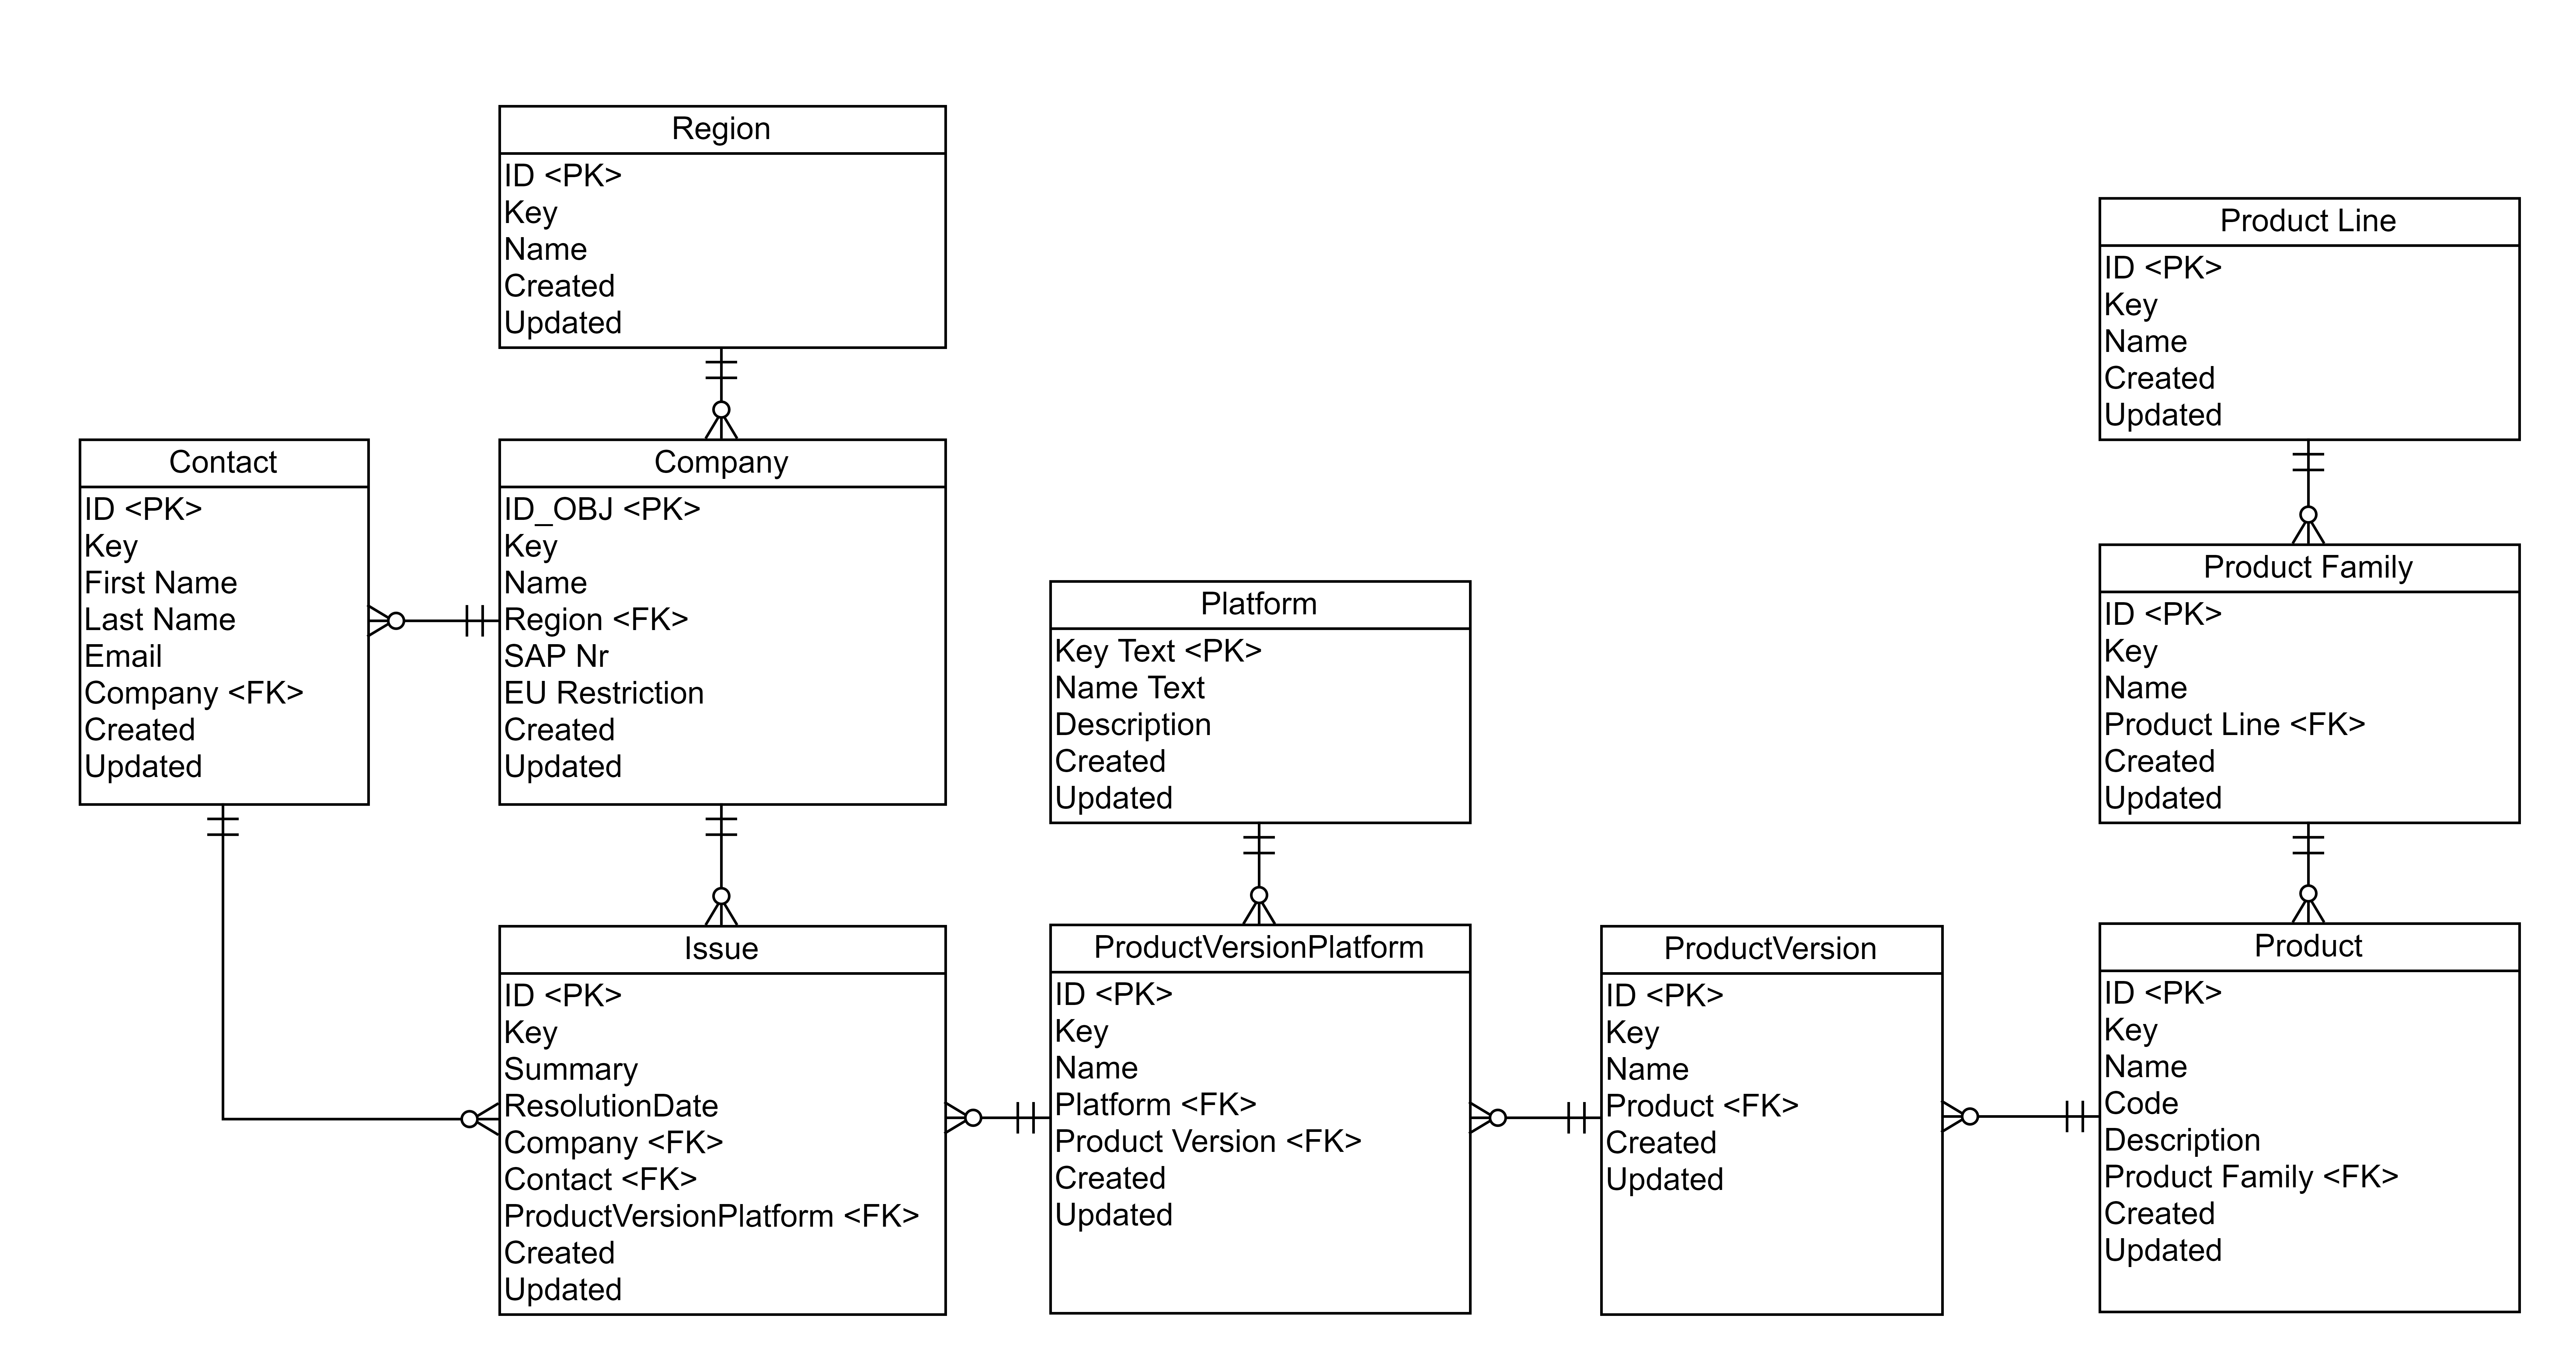
\includegraphics[width=\textwidth]{gfx/data_model.png}
 \caption{Verwendetes Datenmodell für den Prototyp}
\label{fig:praktischeUmsetzung:dataModel}
\end{figure}

\noindent Das gezeigte Datenmodell steht im Zusammenhang mit dem Kundensportsystem \textit{Jira Service Management}. Wenn ein Kunde (\textit{Company}) Probleme mit einem Produkt hat, wird von einer Kontaktperson (\textit{Contact}) ein Support-Ticket (\textit{Issue}) erstellt. Dabei werden alle notwendigen Produktinformationen wie Betriebssystem und Version mit dem \textit{Issue} verknüpft. Weitere Details sind an dieser Stelle nicht relevant und werden dort aufgegriffen, wo es für das Verständnis der Umsetzung sinnvoll ist.

\subsection{Datenbankmigration} \label{subsec:praktischeUmsetzung:Datenmigration}
Zu Beginn soll die Datenbank, die dem nachgestellten \acp{dwh} entspricht, aus dem on-premise SQL Server zu der \textit{Azure SQL Database} migriert werden. 

Für den Migrationsprozess wurden drei mögliche Optionen betrachtet \cite{soh_microsoft_2020}: 
\begin{enumerate}
\item \textbf{1. Bacpac} ...
\item \textbf{\ac{dma}} ist ein Tool, das bewertet, wie gut eine Datenbank für die Migration in die Cloud geeignet ist und gibt einen Überblick, welche Funktionalitäten nicht übernommen werden können. Daneben gibt es die hier relevantere Funktion, das Datenbankschema und anschließend die Daten nach Azure zu übertragen. Für Migrationen im großen Maßstab sollte jedoch die folgende Software bevorzugt werden. 
\item \textbf{Azure Database Migration Service} kann die Daten nicht nur von der on-premise Datenbank in eine Cloud Datenbank übertragen, sondern die Daten während und nach der Migration zwischen den beiden Systemen synchronisieren. Damit kann sichergestellt werden, dass neue Daten, die während dem Migrationsprozess gesammelt werden, nicht verloren gehen. Nach einer Übergangszeit wird die Synchronisation beendet. Diese Anwendung setzt jedoch voraus, dass das korrekte Datenbankschema bereits in der Zieldatenbank vorhanden ist und kann dieses nicht wie der \ac{dma} übertragen. Daher kann es empfehlenswert sein, beide Anwendungen zu kombinieren.
\end{enumerate}

\textit{Data Migration Assistant...}

Die Durchführung beginnt mit der Installation des \ac{dma} auf dem gleichen Server wie die on-premise Datenbank. Für den Zeitraum der Migration wird außerdem die IP-Adresse des Servers in den Firewall-Einstellungen der Azure SQL Datenbank zugelassen. Anschließend wird der \ac{dma} geöffnet und der Migrationsprozess kann über die Benutzeroberfläche durchgeführt werden. Hierzu gehört die Angabe der Quell- und Zielserveradressen, Authentifizierungsinformationen und anschließend die Angabe der zu migrierenden Datenbank. Durch die Hub-and-Spoke-Architektur stehen hier mehrere zur Auswahl. Da sich alle Rohdaten in dem \textit{Hub}, welcher das \ac{dwh} abbildet, befinden, muss nur eine Datenbank migriert werden. Die \textit{Spokes} werden nicht übertragen, weil diese für das aktuelle Reportingframework entworfen wurden, welches durch \textit{Power BI} abgelöst wird. Anschließend wird automatisch ein SQL-Skript erstellt, welches das on-premise Datenbankschema erstellen kann. Dieses kann bei Bedarf angepasst werden und anschließend auf der Zieldatenbank ausgeführt werden. Dies hat hier nur wenige Sekunden gedauert. Abschließend können die Daten in die soeben erstellten Tabellen übertragen werden, wobei die Anwendung den Fortschritt für jede Tabelle in Prozent anzeigt. Die Übertragung der 1,3 GB Daten hat ca. 50 Sekunden benötigt. Es kann also davon ausgegangen werden, dass die Migration der vollen 500 GB wie angenommen in deutlich weniger als einem Tag durchgeführt werden kann. Daraus folgt, dass der \ac{dma} nicht nur für den Prototyp ausreicht, sondern auch für den Umstieg des vollständigen \acp{dwh} geeignet ist.

Neben der Übertragung der Daten ist auch die langfristige Erhaltung der Datenqualität wichtig. Im on-premise SQL-Server werden hierfür Stored Procedures verwendet, welche über einen \textit{Job Agent} täglich ausgeführt werden. Diese führen Plausibilitätschecks durch und suchen nach Unstimmigkeiten, beispielsweise Duplikate oder ungültige Werte wie eine negative Bearbeitungszeit. Wenn eine Auffälligkeit gefunden wird, wird ein Verantwortlicher per E-Mail benachrichtigt, der anschließend die Fehlerursache finden und beheben kann. Die Stored Procedures können problemlos als Bestandteil des Datenbankschemas migriert werden. Die \textit{Azure SQL Datenbank} verfügt jedoch nicht über den \textit{Job Agent}, weswegen die regelmäßige Ausführung der Qualitätschecks anders gelöst werden muss. Eine naheliegende Lösung wäre die Verwendung von \textit{Azure Functions}, da diese über einen Timer getriggert werden können, um dann die Stored Procedures auszuführen. Durch die Kombination mit dem \textit{Azure Monitor} können so gleichzeitig mit wenig Aufwand Logging der Qualitätschecks und Benachrichtigungen bei Problemen umgesetzt werden. Eine konkrete Umsetzung soll hier nicht vorgestellt werden, da die technisch relevanten Aspekte im Abschnitt zur Implementierung des \ac{etl}-Prozesses abgedeckt werden.

\subsection{Implementierung ETL}

\subsection{Erstellen und Bereitstellen von Reports}
Die Reports sind die Schnittstelle zum Endnutzer und präsentiert Auswertungen, die unter anderen als Entscheidungshilfe genutzt werden. Im neuen BI-System sollen diese mit \textit{Power BI} erstellt werden. Dabei soll \textit{Power BI} nicht nur für die Visualisierungen verwendet werden, sondern auch für Auswertungen und Transformationen, die vorher mit \textit{Data Marts} und \textit{T-SQL} durchgeführt wurden. Für den Umstieg zum neuen BI-System bedeutet dies, dass das Reporting vollständig neu implementiert werden muss. Deswegen soll für den Prototyp ein Report erstellt werden, der hierfür alle relevanten Komponenten (Tabelle, Filter, Linien- und Balkendiagramm) enthält.

Der erste Schritt ist das Erstellen eines \textit{Datasets}. Dafür werden die Verbindungsinformationen zur \textit{Azure SQL-Database} angegeben und es wird die Option \textit{Import} gewählt. Das bedeutet, dass die Daten nach \textit{Power BI} gedownloadet werden. Die Alternative \textit{DirectQuery} lädt Daten direkt aus der Datenbank und ist dadurch immer aktuell, würde jedoch zu längeren Ladezeiten der Report führen. Anschließend kann das Datenmodell mit dem \textit{Power Query Editor} angepasst werden. Tabellen und Spalten könnten umbenannt werden, oder Datentypen geändert. Hier soll eine neue Spalte zu der Tabelle \textit{Issue} hinzugefügt werden, die das Alter enthält. Das Alter für einen ungelösten \textit{Issue} ist die Zeit von Erstellung bis zum aktuellen Tag oder für einen gelösten bis zum Lösungszeitpunkt. Ob ein \textit{Issue} in Bearbeitung ist, oder bereits gelöst wurde, kann abhängig davon, ob das \textit{ResolutionDate} gesetzt ist, erkannt werden. Dies wird mit einer IF-Funktion geprüft, die die Bedingung als erstes Argument erhält. Ist die Bedingung wahr, wird das zweite Argument, ansonsten das dritte Argument ausgeführt. In beiden Fällen wird über eine Funktion die Zeitdifferenz in Bezug zum Erstellungszeitpunkt berechnet.

\begin{lstlisting}[frame=single,caption={Code zur Defintion der Spalte \textit{Age}} von Tabelle \textit{Issue},captionpos=b]
Age = 
IF('issue'[ResolutionDate] = BLANK(),
    DATEDIFF('issue'[Created], NOW(), DAY),   
    DATEDIFF('issue'[Created], 'issue'[ResolutionDate], DAY)
)
\end{lstlisting}

\noindent Nachdem die neue Spaltendefinition gespeichert wurde, wird jede Zeile der Tabelle automatisch um den neuen Wert ergänzt. Zusätzlich wird eine neue Tabelle \textit{Calendar} mit \textit{DAX} definiert, die jedes Datum vom Erstellungszeitpunkt des ersten \textit{Issues} bis zum aktuellen Tag enthält. Diese Daten werden hier für eine Zeitachse benötigt. Im nächsten Schritt ist es notwendig, die Beziehungen der Tabellen miteinander zu bearbeiten. Diese sind besonders für das korrekte Filtern in den Reports wichtig. Beziehungen können über die Benutzeroberfläche hinzugefügt werden, in dem Primär- und Fremdschlüssel und die Kardinalität angegeben werden. Nach der Bearbeitung entsprechen die Beziehungen in \textit{Power BI} dem Datenmodell in Abbildung~\ref{fig:praktischeUmsetzung:dataModel}. Damit ist das \textit{Dataset} bereit für die Verwendung in einem Report.

Zu Begin wird ein \textit{Slicer} hinzugefügt, mit dem der Benutzer alle Visualisierungen interaktiv nach Region filtern kann. Dadruch, dass \textit{Power BI} die Beziehungen zwischen den Tabellen kennt, ist die Umsetzung sehr einfach und kann vollständig per Drag-And-Drop durchgeführt werden. Der \textit{Slicer} muss lediglich an die gewünschte Stelle gezogen werden und bekommt das Feld \textit{Name} von \textit{Region} zugewiesen. Jetzt kann ein Nutzer den Report per Dropdown-Filter auf eine Region beschränken.

Die manuell hinzugefügten Spalte \textit{Age} soll in einem Balkendiagramm verwendet werden, dass das durchschnittliche Alter eines \textit{Issues} nach Produktfamilie angibt.

Die nächste Visualisierung soll in einem Liniendiagramm den zeitlichen Verlauf der Anzahl an neu erstellten, geschlossenen und offenen \textit{Issues} anzeigen. Dazu werden der Tabelle \textit{Calendar} drei \textit{Measures} hinzugefügt.  \textit{Measures} werden ebenfalls mit \textit{DAX} definiert und können beispielsweise für Aggregationen in den Visualisierungen verwendet werden. Im Gegensatz zu einer berechneten Spalte, wie \textit{Age}, werden die Ergebnisse von \textit{Measures} nicht im \textit{Dataset} gespeichert, sondern jedes Mal beim Laden des Reports berechnet.

Nach der Implementierung des Reports mit der \textit{Power BI Desktop} Anwendung kann dieser in einen \textit{Workspace} veröffentlicht werden. Danach ist der Report als auch das \textit{Dataset} für alle berechtigten Mitarbeiter über den Webbrowser verfügbar. Die Zugriffsberechtigung auf einen \textit{Workspace} kann über \ac{rbac} und dem \ac{aad} gesteuert werden. Falls eine granulare Zugriffskontrolle erforderlich ist, sollte jedoch die \textit{row-level security} verwendet werden. Mit dieser können Benutzern oder Gruppen \textit{DAX}-Filter zugeordnet werden, die einschränken, welche Inhalte gesehen werden können. Hier ermöglicht diese Funktionalität, dass der erstellte Report mit allen Mitarbeitern geteilt werden kann und gleichzeitig Daten, bei denen es durch die DSGVO notwendig ist, nur von Personen mit europäischem Standort gesehen werden kann.

Der letzte Schritt ist das Einrichten eines Zeitplans für die Aktualisierung des \textit{Datasets}. Mit \textit{Power BI Pro} ist die Anzahl der Aktualisierungen auf achtmal täglich beschränkt, was bezüglich der Anforderungen der kritischste Nachteil gegenüber \textit{Power BI Premium} ist. Ob die Einschränkung, dass Reports nur alle drei Stunden, statt stündlich aktualisiert werden können, den zusätzlich Kosten von \textit{Power BI Premium} rechtfertigen würde, ist abhängig davon, wie kritisch die Aktualität der Reports ist. Da bezüglich der Performance keine Probleme festgestellt wurden und das on-premise BI-System nur einmal täglich aktualisiert wird, kann davon ausgegangen, dass \textit{Power BI Pro} ausreichend ist. Ein Umstieg auf \textit{Premium} wäre außerdem zukünftig jederzeit möglich. 

% self service


\cite[vgl.][]{pearson_pro_2020}

% refreshs/direct query

\subsection{Einrichtung der Datengovernance}
Zum Verwenden von \textit{Azure Purview} für die Datengovernance, muss der Dienst zunächst eingerichtet werden. Dazu öffnet ein berechtigter Nutzer die Webanwendung \textit{Purview Studio}. Als Erstes werden dort die Ressourcen, die gescannt werden sollen, registriert, indem die entsprechenden Verbindungsinformationen angegeben werden.Der Prototyp beschränkt sich hierbei auf die \textit{SQL-Database}. Nun kann beim Erstellen eines sogenannten \textit{Scans}, die zuvor eingerichtete \textit{Self hosted-integration runtime} und die \textit{SQL-Database} angegeben werden. Daneben ist noch die Verlinkung mit dem Passwort des Dienstprinzipals im \textit{Key Vault} notwendig. Nach einem erfolgreichen Verbindungstest kann abschließend ein Zeitplan für regelmäßige Ausführungen des \textit{Scans} definiert werden, oder alternativ eine einmalige Ausführung gestartet werden. Während für den Prototyp letztere Option gewählt wurde, ist für ein zukünftiges Cloud-BI-System eine regelmäßige Wiederholung zu bevorzugen, damit die gesammelten Metadaten aktuell bleiben. 

Nachdem der \textit{Scan} durchgeführt wurde, können die gesammelten Erkenntnisse erkundet werden. Dazu gehört zum Beispiel eine Übersicht über alle Tabellen und Spalten inklusive des Datentyps. Vom besonderen Interesse ist die Klassifizierung der Spalten, welche anhand einer Vielzahl von vordefinierten Regeln erfolgt. Diese Klassifizierungsregeln basieren entweder auf Wörterbüchern oder RegEx-Pattern und können damit unter anderem US-Sozialversicherungsnummern oder Bankleitzahlen erkennen. Auch das Hinzufügen von benutzerdefinierten Klassifizierungsregeln ist möglich. Kann der Wert einer Spalte zu einer Klassifizierungsregel zugeordnet werden, speichert \textit{Purview} eine entsprechende Klassifizierung, jedoch nicht den eigentlichen Wert. Für den Prototyp konnte damit eine einzige Klassifizierung gefunden werden, nämlich dass die Tabelle \textit{Contact} eine Spalte mit E-Mail-Adressen enthält. Hieran ist zumindest zu erkennen, dass das Grundkonzept funktioniert, denn weitere Erkenntnisse waren bei dem vereinfachten Datenmodell nicht zu erwarten. Es muss jedoch angemerkt werden, dass diese Art von Klassifizierung sich nicht vollständig mit der dazugehörigen Anforderung deckt. In dieser wurde beschrieben, dass die  Daten bezüglich ihrer Vertraulichkeit klassifiziert werden sollen. Also nicht nach ihrem konkreten Inhalt, wie es bei \textit{Purview} der Fall ist. Dieses Problem könnte zum Beispiel durch die Funktion \textit{Sensitivitätskennzeichnungen} gelöst werden, welche sich aktuell in der Vorschauphase befindet. Da die Anforderung nicht die höchste Priorität hat und ein kurzzeitiger Ausfall der Funktionalität nicht kritisch für das operative Tagesgeschäft ist, wäre die Verwendung der Vorschau hier akzeptabel. Denn dann ist es möglich, basierend auf den gefundenen Klassifizierungen, automatisch \textit{Sensitivitätskennzeichnungen} zu den Metadaten hinzuzufügen. Wenn die Klassifizierungsregeln so festgelegt werden, dass aus bestimmten Kombinationen eine eindeutige Vertraulichkeit abgeleitet werden kann, wäre so ein vollständiges Erfüllen der Anforderung möglich. 

Europäische Kunden verfügen über das \textit{Recht auf Vergessenwerden}, das innerhalb von 30 Tagen ausgeführt werden muss. Beim Finden aller Daten, die dann gelöscht werden müssen, kann Purview sehr hilfreich sein. In dem eine benutzerdefinierte Klassifizierungsregel angelegt wird, die bei eindeutigen Kundenkennzeichnungen greift, wie beispielsweise dem Namen oder der SAP-Nummer, können mit einem erneuten \textit{Scan} alle Tabellen und Reports mit Daten des Kunden gefunden werden. Dadurch wird das Risiko, dass Daten beim Durchführen der Löschung übersehen werden, minimiert.

Die von der DSGVO geforderte Datenflussdokumentation kann zwischen den Datenbanktabellen und den einzelnen Reports in \textit{Power BI} automatisch erstellt werden, in dem \textit{Power BI} als weitere Quelle für die \textit{Scans} registriert wird. Somit ist es möglich, schnell herauszufinden, welche Tabellen in welchen Reports verwendet werden. Die Datenintegration mit \textit{Azure Functions} wird allerdings nicht dokumentiert, da diese nur mit der \textit{Azure Data Factory} berücksichtigt werden kann. Demnach handelt es sich hier um eine weitere Anforderung, die mit Purview nur teilweise erfüllt werden kann. Aus diesem Grund \textit{Azure Functions} mit der \textit{Data Factory} zu ersetzen erscheint jedoch nicht sinnvoll, da dann weitere \acp{vm} notwendig wären, wodurch Kosten und Wartungsaufwand steigen. Da sich die Quellsysteme grundsätzlich selten verändern, wäre es voraussichtlich zeitsparender, die Dokumentation der Datenintegration manuell zu pflegen. Das ist über die REST API von \textit{Purview} möglich. Dies würde immer noch den Mehrwert bieten, dass die vollständige Dokumentation aller Datenflüsse an einem Ort gefunden werden kann. Außerdem dürfen die meisten Nutzer Reports erstellen, während der ETL-Prozess nur von einer kleinen Gruppe verändert werden kann. Daher sollte die Verwendung dieser Funktion insgesamt als positiv bewertet werden. \cite[vgl.][]{lesteve_definitive_2021, msdoc_22_purview_sensLabel, riscutia_data_2021, borosch_cloud_2021}

Zusammengefasst konnte durch die praktische Verwendung von \textit{Azure Purview} festgestellt werden, dass dieser Dienst zwar hilfreich bei der Erfüllung von DSGVO-Vorgaben ist und einen guten Überblick über die Datenlandschaft im BI-System geben kann, jedoch müssen bezüglich der Anforderungen Kompromisse eingegangen werden, die durch die mangelnden Alternativen jedoch akzeptabel sind.

\subsection{Auswertung von Personendaten mit expliziter Zustimmung des Betriebsrates}

\subsection{Einbindung von Azure Machine Learning für fortgeschrittene Analysen}